\documentclass[1p]{elsarticle_modified}
%\bibliographystyle{elsarticle-num}

%\usepackage[colorlinks]{hyperref}
%\usepackage{abbrmath_seonhwa} %\Abb, \Ascr, \Acal ,\Abf, \Afrak
\usepackage{amsfonts}
\usepackage{amssymb}
\usepackage{amsmath}
\usepackage{amsthm}
\usepackage{scalefnt}
\usepackage{amsbsy}
\usepackage{kotex}
\usepackage{caption}
\usepackage{subfig}
\usepackage{color}
\usepackage{graphicx}
\usepackage{xcolor} %% white, black, red, green, blue, cyan, magenta, yellow
\usepackage{float}
\usepackage{setspace}
\usepackage{hyperref}

\usepackage{tikz}
\usetikzlibrary{arrows}

\usepackage{multirow}
\usepackage{array} % fixed length table
\usepackage{hhline}

%%%%%%%%%%%%%%%%%%%%%
\makeatletter
\renewcommand*\env@matrix[1][\arraystretch]{%
	\edef\arraystretch{#1}%
	\hskip -\arraycolsep
	\let\@ifnextchar\new@ifnextchar
	\array{*\c@MaxMatrixCols c}}
\makeatother %https://tex.stackexchange.com/questions/14071/how-can-i-increase-the-line-spacing-in-a-matrix
%%%%%%%%%%%%%%%

\usepackage[normalem]{ulem}

\newcommand{\msout}[1]{\ifmmode\text{\sout{\ensuremath{#1}}}\else\sout{#1}\fi}
%SOURCE: \msout is \stkout macro in https://tex.stackexchange.com/questions/20609/strikeout-in-math-mode

\newcommand{\cancel}[1]{
	\ifmmode
	{\color{red}\msout{#1}}
	\else
	{\color{red}\sout{#1}}
	\fi
}

\newcommand{\add}[1]{
	{\color{blue}\uwave{#1}}
}

\newcommand{\replace}[2]{
	\ifmmode
	{\color{red}\msout{#1}}{\color{blue}\uwave{#2}}
	\else
	{\color{red}\sout{#1}}{\color{blue}\uwave{#2}}
	\fi
}

\newcommand{\Sol}{\mathcal{S}} %segment
\newcommand{\D}{D} %diagram
\newcommand{\A}{\mathcal{A}} %arc


%%%%%%%%%%%%%%%%%%%%%%%%%%%%%5 test

\def\sl{\operatorname{\textup{SL}}(2,\Cbb)}
\def\psl{\operatorname{\textup{PSL}}(2,\Cbb)}
\def\quan{\mkern 1mu \triangleright \mkern 1mu}

\theoremstyle{definition}
\newtheorem{thm}{Theorem}[section]
\newtheorem{prop}[thm]{Proposition}
\newtheorem{lem}[thm]{Lemma}
\newtheorem{ques}[thm]{Question}
\newtheorem{cor}[thm]{Corollary}
\newtheorem{defn}[thm]{Definition}
\newtheorem{exam}[thm]{Example}
\newtheorem{rmk}[thm]{Remark}
\newtheorem{alg}[thm]{Algorithm}

\newcommand{\I}{\sqrt{-1}}
\begin{document}

%\begin{frontmatter}
%
%\title{Boundary parabolic representations of knots up to 8 crossings}
%
%%% Group authors per affiliation:
%\author{Yunhi Cho} 
%\address{Department of Mathematics, University of Seoul, Seoul, Korea}
%\ead{yhcho@uos.ac.kr}
%
%
%\author{Seonhwa Kim} %\fnref{s_kim}}
%\address{Center for Geometry and Physics, Institute for Basic Science, Pohang, 37673, Korea}
%\ead{ryeona17@ibs.re.kr}
%
%\author{Hyuk Kim}
%\address{Department of Mathematical Sciences, Seoul National University, Seoul 08826, Korea}
%\ead{hyukkim@snu.ac.kr}
%
%\author{Seokbeom Yoon}
%\address{Department of Mathematical Sciences, Seoul National University, Seoul, 08826,  Korea}
%\ead{sbyoon15@snu.ac.kr}
%
%\begin{abstract}
%We find all boundary parabolic representation of knots up to 8 crossings.
%
%\end{abstract}
%\begin{keyword}
%    \MSC[2010] 57M25 
%\end{keyword}
%
%\end{frontmatter}

%\linenumbers
%\tableofcontents
%
\newcommand\colored[1]{\textcolor{white}{\rule[-0.35ex]{0.8em}{1.4ex}}\kern-0.8em\color{red} #1}%
%\newcommand\colored[1]{\textcolor{white}{ #1}\kern-2.17ex	\textcolor{white}{ #1}\kern-1.81ex	\textcolor{white}{ #1}\kern-2.15ex\color{red}#1	}

{\Large $\underline{12a_{0926}~(K12a_{0926})}$}

\setlength{\tabcolsep}{10pt}
\renewcommand{\arraystretch}{1.6}
\vspace{1cm}\begin{tabular}{m{100pt}>{\centering\arraybackslash}m{274pt}}
\multirow{5}{120pt}{
	\centering
	\includegraphics[width=112pt]{../../../GIT/diagram.site/Diagrams/png/1727_12a_0926.png}\\
\ \ \ A knot diagram\footnotemark}&
\allowdisplaybreaks
\textbf{Linearized knot diagam} \\
\cline{2-2}
 &
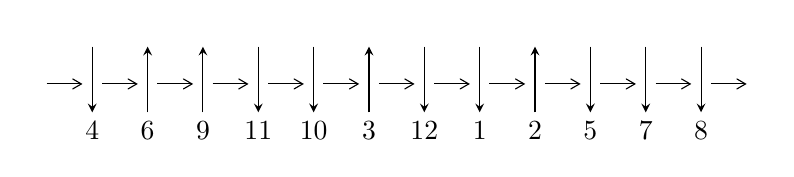
\begin{tikzpicture}[x=20pt, y=17pt]
	% nodes
	\node (C0) at (0, 0) {};
	\node (C1) at (1, 0) {};
	\node (C1U) at (1, +1) {};
	\node (C1D) at (1, -1) {4};

	\node (C2) at (2, 0) {};
	\node (C2U) at (2, +1) {};
	\node (C2D) at (2, -1) {6};

	\node (C3) at (3, 0) {};
	\node (C3U) at (3, +1) {};
	\node (C3D) at (3, -1) {9};

	\node (C4) at (4, 0) {};
	\node (C4U) at (4, +1) {};
	\node (C4D) at (4, -1) {11};

	\node (C5) at (5, 0) {};
	\node (C5U) at (5, +1) {};
	\node (C5D) at (5, -1) {10};

	\node (C6) at (6, 0) {};
	\node (C6U) at (6, +1) {};
	\node (C6D) at (6, -1) {3};

	\node (C7) at (7, 0) {};
	\node (C7U) at (7, +1) {};
	\node (C7D) at (7, -1) {12};

	\node (C8) at (8, 0) {};
	\node (C8U) at (8, +1) {};
	\node (C8D) at (8, -1) {1};

	\node (C9) at (9, 0) {};
	\node (C9U) at (9, +1) {};
	\node (C9D) at (9, -1) {2};

	\node (C10) at (10, 0) {};
	\node (C10U) at (10, +1) {};
	\node (C10D) at (10, -1) {5};

	\node (C11) at (11, 0) {};
	\node (C11U) at (11, +1) {};
	\node (C11D) at (11, -1) {7};

	\node (C12) at (12, 0) {};
	\node (C12U) at (12, +1) {};
	\node (C12D) at (12, -1) {8};
	\node (C13) at (13, 0) {};

	% arrows
	\draw[->,>={angle 60}]
	(C0) edge (C1) (C1) edge (C2) (C2) edge (C3) (C3) edge (C4) (C4) edge (C5) (C5) edge (C6) (C6) edge (C7) (C7) edge (C8) (C8) edge (C9) (C9) edge (C10) (C10) edge (C11) (C11) edge (C12) (C12) edge (C13) ;	\draw[->,>=stealth]
	(C1U) edge (C1D) (C2D) edge (C2U) (C3D) edge (C3U) (C4U) edge (C4D) (C5U) edge (C5D) (C6D) edge (C6U) (C7U) edge (C7D) (C8U) edge (C8D) (C9D) edge (C9U) (C10U) edge (C10D) (C11U) edge (C11D) (C12U) edge (C12D) ;
	\end{tikzpicture} \\
\hhline{~~} \\& 
\textbf{Solving Sequence} \\ \cline{2-2} 
 &
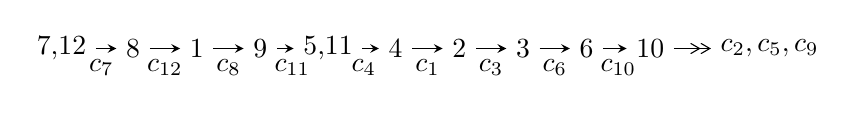
\begin{tikzpicture}[x=23pt, y=7pt]
	% node
	\node (A0) at (-1/8, 0) {7,12};
	\node (A1) at (1, 0) {8};
	\node (A2) at (2, 0) {1};
	\node (A3) at (3, 0) {9};
	\node (A4) at (65/16, 0) {5,11};
	\node (A5) at (41/8, 0) {4};
	\node (A6) at (49/8, 0) {2};
	\node (A7) at (57/8, 0) {3};
	\node (A8) at (65/8, 0) {6};
	\node (A9) at (73/8, 0) {10};
	\node (C1) at (1/2, -1) {$c_{7}$};
	\node (C2) at (3/2, -1) {$c_{12}$};
	\node (C3) at (5/2, -1) {$c_{8}$};
	\node (C4) at (7/2, -1) {$c_{11}$};
	\node (C5) at (37/8, -1) {$c_{4}$};
	\node (C6) at (45/8, -1) {$c_{1}$};
	\node (C7) at (53/8, -1) {$c_{3}$};
	\node (C8) at (61/8, -1) {$c_{6}$};
	\node (C9) at (69/8, -1) {$c_{10}$};
	\node (A10) at (11, 0) {$c_{2},c_{5},c_{9}$};

	% edge
	\draw[->,>=stealth]	
	(A0) edge (A1) (A1) edge (A2) (A2) edge (A3) (A3) edge (A4) (A4) edge (A5) (A5) edge (A6) (A6) edge (A7) (A7) edge (A8) (A8) edge (A9) ;
	\draw[->>,>={angle 60}]	
	(A9) edge (A10);
\end{tikzpicture} \\ 

\end{tabular} \\

\footnotetext{
The image of knot diagram is generated by the software ``\textbf{Draw programme}" developed by Andrew Bartholomew(\url{http://www.layer8.co.uk/maths/draw/index.htm\#Running-draw}), where we modified some parts for our purpose(\url{https://github.com/CATsTAILs/LinksPainter}).
}\phantom \\ \newline 
\centering \textbf{Ideals for irreducible components\footnotemark of $X_{\text{par}}$} 
 
\begin{align*}
I^u_{1}&=\langle 
8.47533\times10^{71} u^{79}+3.31160\times10^{71} u^{78}+\cdots+2.05866\times10^{72} b-2.65713\times10^{72},\\
\phantom{I^u_{1}}&\phantom{= \langle  }-7.84336\times10^{72} u^{79}-1.83623\times10^{73} u^{78}+\cdots+1.85280\times10^{73} a-1.38382\times10^{73},\;u^{80}+u^{79}+\cdots+2 u+1\rangle \\
I^u_{2}&=\langle 
- u^{15}-2 u^{14}+\cdots+b+2,\;2 u^{16}-3 u^{15}+\cdots+a+8,\;u^{17}-11 u^{15}+\cdots+2 u+1\rangle \\
\\
\end{align*}
\raggedright * 2 irreducible components of $\dim_{\mathbb{C}}=0$, with total 97 representations.\\
\footnotetext{All coefficients of polynomials are rational numbers. But the coefficients are sometimes approximated in decimal forms when there is not enough margin.}
\newpage
\renewcommand{\arraystretch}{1}
\centering \section*{I. $I^u_{1}= \langle 8.48\times10^{71} u^{79}+3.31\times10^{71} u^{78}+\cdots+2.06\times10^{72} b-2.66\times10^{72},\;-7.84\times10^{72} u^{79}-1.84\times10^{73} u^{78}+\cdots+1.85\times10^{73} a-1.38\times10^{73},\;u^{80}+u^{79}+\cdots+2 u+1 \rangle$}
\flushleft \textbf{(i) Arc colorings}\\
\begin{tabular}{m{7pt} m{180pt} m{7pt} m{180pt} }
\flushright $a_{7}=$&$\begin{pmatrix}1\\0\end{pmatrix}$ \\
\flushright $a_{12}=$&$\begin{pmatrix}0\\u\end{pmatrix}$ \\
\flushright $a_{8}=$&$\begin{pmatrix}1\\u^2\end{pmatrix}$ \\
\flushright $a_{1}=$&$\begin{pmatrix}- u\\- u^3+u\end{pmatrix}$ \\
\flushright $a_{9}=$&$\begin{pmatrix}- u^2+1\\- u^4+2 u^2\end{pmatrix}$ \\
\flushright $a_{5}=$&$\begin{pmatrix}0.423326 u^{79}+0.991058 u^{78}+\cdots-9.58238 u+0.746882\\-0.411691 u^{79}-0.160862 u^{78}+\cdots-1.54970 u+1.29071\end{pmatrix}$ \\
\flushright $a_{11}=$&$\begin{pmatrix}u\\u\end{pmatrix}$ \\
\flushright $a_{4}=$&$\begin{pmatrix}0.609160 u^{79}+0.709751 u^{78}+\cdots-8.11356 u+1.06379\\-0.225856 u^{79}-0.442169 u^{78}+\cdots-0.0808800 u+1.60761\end{pmatrix}$ \\
\flushright $a_{2}=$&$\begin{pmatrix}-0.652505 u^{79}+1.32207 u^{78}+\cdots-10.5607 u+0.0192152\\-0.943472 u^{79}+0.111525 u^{78}+\cdots-3.28103 u+0.0878461\end{pmatrix}$ \\
\flushright $a_{3}=$&$\begin{pmatrix}0.862772 u^{79}+0.642394 u^{78}+\cdots-7.88631 u+0.131545\\0.0159171 u^{79}-0.185399 u^{78}+\cdots-0.538693 u+1.44431\end{pmatrix}$ \\
\flushright $a_{6}=$&$\begin{pmatrix}1.11988 u^{79}+0.492728 u^{78}+\cdots-4.34134 u+2.80234\\0.596804 u^{79}+0.790725 u^{78}+\cdots-2.03464 u+1.22731\end{pmatrix}$ \\
\flushright $a_{10}=$&$\begin{pmatrix}-2.19980 u^{79}-0.534214 u^{78}+\cdots+5.11355 u-0.488944\\-1.56332 u^{79}+0.378993 u^{78}+\cdots+3.09382 u-0.595903\end{pmatrix}$\\&\end{tabular}
\flushleft \textbf{(ii) Obstruction class $= -1$}\\~\\
\flushleft \textbf{(iii) Cusp Shapes $= 0.629075 u^{79}+3.23575 u^{78}+\cdots-28.6021 u+0.810717$}\\~\\
\newpage\renewcommand{\arraystretch}{1}
\flushleft \textbf{(iv) u-Polynomials at the component}\newline \\
\begin{tabular}{m{50pt}|m{274pt}}
Crossings & \hspace{64pt}u-Polynomials at each crossing \\
\hline $$\begin{aligned}c_{1}\end{aligned}$$&$\begin{aligned}
&u^{80}-13 u^{79}+\cdots+1636 u-233
\end{aligned}$\\
\hline $$\begin{aligned}c_{2},c_{6}\end{aligned}$$&$\begin{aligned}
&u^{80}-31 u^{78}+\cdots+4811 u-917
\end{aligned}$\\
\hline $$\begin{aligned}c_{3}\end{aligned}$$&$\begin{aligned}
&u^{80}- u^{79}+\cdots+55 u-43
\end{aligned}$\\
\hline $$\begin{aligned}c_{4},c_{5},c_{10}\end{aligned}$$&$\begin{aligned}
&u^{80}- u^{79}+\cdots-26 u+1
\end{aligned}$\\
\hline $$\begin{aligned}c_{7},c_{8},c_{11}\\c_{12}\end{aligned}$$&$\begin{aligned}
&u^{80}- u^{79}+\cdots-2 u+1
\end{aligned}$\\
\hline $$\begin{aligned}c_{9}\end{aligned}$$&$\begin{aligned}
&u^{80}+2 u^{79}+\cdots+105006 u+58531
\end{aligned}$\\
\hline
\end{tabular}\\~\\
\newpage\renewcommand{\arraystretch}{1}
\flushleft \textbf{(v) Riley Polynomials at the component}\newline \\
\begin{tabular}{m{50pt}|m{274pt}}
Crossings & \hspace{64pt}Riley Polynomials at each crossing \\
\hline $$\begin{aligned}c_{1}\end{aligned}$$&$\begin{aligned}
&y^{80}-9 y^{79}+\cdots-1784106 y+54289
\end{aligned}$\\
\hline $$\begin{aligned}c_{2},c_{6}\end{aligned}$$&$\begin{aligned}
&y^{80}-62 y^{79}+\cdots-33892961 y+840889
\end{aligned}$\\
\hline $$\begin{aligned}c_{3}\end{aligned}$$&$\begin{aligned}
&y^{80}+11 y^{79}+\cdots+14347 y+1849
\end{aligned}$\\
\hline $$\begin{aligned}c_{4},c_{5},c_{10}\end{aligned}$$&$\begin{aligned}
&y^{80}+83 y^{79}+\cdots-450 y+1
\end{aligned}$\\
\hline $$\begin{aligned}c_{7},c_{8},c_{11}\\c_{12}\end{aligned}$$&$\begin{aligned}
&y^{80}-95 y^{79}+\cdots-28 y+1
\end{aligned}$\\
\hline $$\begin{aligned}c_{9}\end{aligned}$$&$\begin{aligned}
&y^{80}-34 y^{79}+\cdots-99189866468 y+3425877961
\end{aligned}$\\
\hline
\end{tabular}\\~\\
\newpage\flushleft \textbf{(vi) Complex Volumes and Cusp Shapes}
$$\begin{array}{c|c|c}  
\text{Solutions to }I^u_{1}& \I (\text{vol} + \sqrt{-1}CS) & \text{Cusp shape}\\
 \hline 
\begin{aligned}
u &= -0.897708 + 0.453066 I \\
a &= \phantom{-}0.53900 + 1.82561 I \\
b &= \phantom{-}1.167400 + 0.634500 I\end{aligned}
 & \phantom{-}2.78959 + 1.45843 I & \phantom{-0.000000 } 0 \\ \hline\begin{aligned}
u &= -0.897708 - 0.453066 I \\
a &= \phantom{-}0.53900 - 1.82561 I \\
b &= \phantom{-}1.167400 - 0.634500 I\end{aligned}
 & \phantom{-}2.78959 - 1.45843 I & \phantom{-0.000000 } 0 \\ \hline\begin{aligned}
u &= \phantom{-}0.762672 + 0.629552 I \\
a &= -1.12215 + 1.68586 I \\
b &= -2.34369 + 0.66567 I\end{aligned}
 & \phantom{-}7.9204 - 12.3069 I & \phantom{-0.000000 } 0 \\ \hline\begin{aligned}
u &= \phantom{-}0.762672 - 0.629552 I \\
a &= -1.12215 - 1.68586 I \\
b &= -2.34369 - 0.66567 I\end{aligned}
 & \phantom{-}7.9204 + 12.3069 I & \phantom{-0.000000 } 0 \\ \hline\begin{aligned}
u &= -0.572465 + 0.750938 I \\
a &= -1.17173 - 1.57864 I \\
b &= -2.37823 - 0.70667 I\end{aligned}
 & \phantom{-}3.67383 + 2.53720 I & \phantom{-0.000000 } 0 \\ \hline\begin{aligned}
u &= -0.572465 - 0.750938 I \\
a &= -1.17173 + 1.57864 I \\
b &= -2.37823 + 0.70667 I\end{aligned}
 & \phantom{-}3.67383 - 2.53720 I & \phantom{-0.000000 } 0 \\ \hline\begin{aligned}
u &= -0.773820 + 0.517620 I \\
a &= -0.269244 + 0.677104 I \\
b &= \phantom{-}0.802233 + 0.675829 I\end{aligned}
 & \phantom{-}1.07794 + 8.21292 I & \phantom{-0.000000 } 0 \\ \hline\begin{aligned}
u &= -0.773820 - 0.517620 I \\
a &= -0.269244 - 0.677104 I \\
b &= \phantom{-}0.802233 - 0.675829 I\end{aligned}
 & \phantom{-}1.07794 - 8.21292 I & \phantom{-0.000000 } 0 \\ \hline\begin{aligned}
u &= \phantom{-}0.791077 + 0.464930 I \\
a &= \phantom{-}1.14601 - 1.43541 I \\
b &= \phantom{-}2.08530 - 0.15769 I\end{aligned}
 & \phantom{-}3.22885 - 5.95807 I & \phantom{-0.000000 } 0 \\ \hline\begin{aligned}
u &= \phantom{-}0.791077 - 0.464930 I \\
a &= \phantom{-}1.14601 + 1.43541 I \\
b &= \phantom{-}2.08530 + 0.15769 I\end{aligned}
 & \phantom{-}3.22885 + 5.95807 I & \phantom{-0.000000 } 0\\
 \hline 
 \end{array}$$\newpage$$\begin{array}{c|c|c}  
\text{Solutions to }I^u_{1}& \I (\text{vol} + \sqrt{-1}CS) & \text{Cusp shape}\\
 \hline 
\begin{aligned}
u &= \phantom{-}1.031290 + 0.352939 I \\
a &= \phantom{-}0.585092 - 0.011311 I \\
b &= \phantom{-}0.168013 + 0.347384 I\end{aligned}
 & -0.394182 + 0.525357 I & \phantom{-0.000000 } 0 \\ \hline\begin{aligned}
u &= \phantom{-}1.031290 - 0.352939 I \\
a &= \phantom{-}0.585092 + 0.011311 I \\
b &= \phantom{-}0.168013 - 0.347384 I\end{aligned}
 & -0.394182 - 0.525357 I & \phantom{-0.000000 } 0 \\ \hline\begin{aligned}
u &= -0.614673 + 0.600907 I \\
a &= \phantom{-}0.57482 + 1.46306 I \\
b &= \phantom{-}1.64181 + 0.64625 I\end{aligned}
 & \phantom{-}2.17329 + 2.14394 I & \phantom{-0.000000 } 0 \\ \hline\begin{aligned}
u &= -0.614673 - 0.600907 I \\
a &= \phantom{-}0.57482 - 1.46306 I \\
b &= \phantom{-}1.64181 - 0.64625 I\end{aligned}
 & \phantom{-}2.17329 - 2.14394 I & \phantom{-0.000000 } 0 \\ \hline\begin{aligned}
u &= \phantom{-}0.627888 + 0.556081 I \\
a &= \phantom{-}0.241217 - 0.178544 I \\
b &= \phantom{-}0.438984 - 0.279024 I\end{aligned}
 & -1.22309 - 1.89098 I & \phantom{-0.000000 } 0 \\ \hline\begin{aligned}
u &= \phantom{-}0.627888 - 0.556081 I \\
a &= \phantom{-}0.241217 + 0.178544 I \\
b &= \phantom{-}0.438984 + 0.279024 I\end{aligned}
 & -1.22309 + 1.89098 I & \phantom{-0.000000 } 0 \\ \hline\begin{aligned}
u &= \phantom{-}0.215373 + 0.805835 I \\
a &= -0.456300 + 1.014000 I \\
b &= -2.12939 + 0.26584 I\end{aligned}
 & \phantom{-}9.58477 + 7.55429 I & \phantom{-0.000000 } 0 \\ \hline\begin{aligned}
u &= \phantom{-}0.215373 - 0.805835 I \\
a &= -0.456300 - 1.014000 I \\
b &= -2.12939 - 0.26584 I\end{aligned}
 & \phantom{-}9.58477 - 7.55429 I & \phantom{-0.000000 } 0 \\ \hline\begin{aligned}
u &= -0.746808 + 0.334933 I \\
a &= -0.118659 - 0.117796 I \\
b &= -0.864888 - 0.020645 I\end{aligned}
 & -2.53049 + 3.60833 I & -9.69090 - 7.89703 I \\ \hline\begin{aligned}
u &= -0.746808 - 0.334933 I \\
a &= -0.118659 + 0.117796 I \\
b &= -0.864888 + 0.020645 I\end{aligned}
 & -2.53049 - 3.60833 I & -9.69090 + 7.89703 I\\
 \hline 
 \end{array}$$\newpage$$\begin{array}{c|c|c}  
\text{Solutions to }I^u_{1}& \I (\text{vol} + \sqrt{-1}CS) & \text{Cusp shape}\\
 \hline 
\begin{aligned}
u &= \phantom{-}0.691584 + 0.363567 I \\
a &= \phantom{-}0.90879 - 1.21008 I \\
b &= \phantom{-}0.282684 + 0.028990 I\end{aligned}
 & \phantom{-}1.17370 - 2.56864 I & -1.56142 + 6.00737 I \\ \hline\begin{aligned}
u &= \phantom{-}0.691584 - 0.363567 I \\
a &= \phantom{-}0.90879 + 1.21008 I \\
b &= \phantom{-}0.282684 - 0.028990 I\end{aligned}
 & \phantom{-}1.17370 + 2.56864 I & -1.56142 - 6.00737 I \\ \hline\begin{aligned}
u &= -0.628233 + 0.302083 I \\
a &= \phantom{-}0.05350 + 1.67415 I \\
b &= \phantom{-}0.754684 + 1.015830 I\end{aligned}
 & \phantom{-}1.38631 + 2.18514 I & -0.53306 - 7.27019 I \\ \hline\begin{aligned}
u &= -0.628233 - 0.302083 I \\
a &= \phantom{-}0.05350 - 1.67415 I \\
b &= \phantom{-}0.754684 - 1.015830 I\end{aligned}
 & \phantom{-}1.38631 - 2.18514 I & -0.53306 + 7.27019 I \\ \hline\begin{aligned}
u &= -0.108684 + 0.688204 I \\
a &= -0.071269 + 0.542015 I \\
b &= \phantom{-}0.468950 - 0.513867 I\end{aligned}
 & \phantom{-}3.07552 - 4.18485 I & -0.43694 + 5.65022 I \\ \hline\begin{aligned}
u &= -0.108684 - 0.688204 I \\
a &= -0.071269 - 0.542015 I \\
b &= \phantom{-}0.468950 + 0.513867 I\end{aligned}
 & \phantom{-}3.07552 + 4.18485 I & -0.43694 - 5.65022 I \\ \hline\begin{aligned}
u &= -1.258050 + 0.418420 I \\
a &= -1.03868 - 2.32084 I \\
b &= -1.23958 - 1.24602 I\end{aligned}
 & \phantom{-}5.06105 - 3.22792 I & \phantom{-0.000000 } 0 \\ \hline\begin{aligned}
u &= -1.258050 - 0.418420 I \\
a &= -1.03868 + 2.32084 I \\
b &= -1.23958 + 1.24602 I\end{aligned}
 & \phantom{-}5.06105 + 3.22792 I & \phantom{-0.000000 } 0 \\ \hline\begin{aligned}
u &= \phantom{-}0.667781\phantom{ +0.000000I} \\
a &= \phantom{-}0.487700\phantom{ +0.000000I} \\
b &= -0.209816\phantom{ +0.000000I}\end{aligned}
 & -1.04488\phantom{ +0.000000I} & -9.73780\phantom{ +0.000000I} \\ \hline\begin{aligned}
u &= \phantom{-}0.025531 + 0.645716 I \\
a &= -0.600777 - 0.451263 I \\
b &= \phantom{-}1.62555 - 0.26182 I\end{aligned}
 & \phantom{-}5.51085 + 2.26331 I & \phantom{-}0.63689 - 2.84719 I\\
 \hline 
 \end{array}$$\newpage$$\begin{array}{c|c|c}  
\text{Solutions to }I^u_{1}& \I (\text{vol} + \sqrt{-1}CS) & \text{Cusp shape}\\
 \hline 
\begin{aligned}
u &= \phantom{-}0.025531 - 0.645716 I \\
a &= -0.600777 + 0.451263 I \\
b &= \phantom{-}1.62555 + 0.26182 I\end{aligned}
 & \phantom{-}5.51085 - 2.26331 I & \phantom{-}0.63689 + 2.84719 I \\ \hline\begin{aligned}
u &= -0.525952 + 0.362720 I \\
a &= \phantom{-}0.05531 - 1.50930 I \\
b &= -1.71229 + 0.18267 I\end{aligned}
 & \phantom{-}8.70489 + 4.16019 I & \phantom{-}0.88771 - 7.52875 I \\ \hline\begin{aligned}
u &= -0.525952 - 0.362720 I \\
a &= \phantom{-}0.05531 + 1.50930 I \\
b &= -1.71229 - 0.18267 I\end{aligned}
 & \phantom{-}8.70489 - 4.16019 I & \phantom{-}0.88771 + 7.52875 I \\ \hline\begin{aligned}
u &= \phantom{-}0.543476 + 0.317534 I \\
a &= -1.50383 + 1.71269 I \\
b &= -2.59856 - 0.33649 I\end{aligned}
 & \phantom{-}8.35841 + 1.11561 I & \phantom{-}1.24449 + 2.28226 I \\ \hline\begin{aligned}
u &= \phantom{-}0.543476 - 0.317534 I \\
a &= -1.50383 - 1.71269 I \\
b &= -2.59856 + 0.33649 I\end{aligned}
 & \phantom{-}8.35841 - 1.11561 I & \phantom{-}1.24449 - 2.28226 I \\ \hline\begin{aligned}
u &= \phantom{-}0.584085 + 0.142445 I \\
a &= \phantom{-}0.41745 + 1.57646 I \\
b &= \phantom{-}0.582932 + 0.172246 I\end{aligned}
 & -1.244310 - 0.535370 I & -8.05750 - 1.18114 I \\ \hline\begin{aligned}
u &= \phantom{-}0.584085 - 0.142445 I \\
a &= \phantom{-}0.41745 - 1.57646 I \\
b &= \phantom{-}0.582932 - 0.172246 I\end{aligned}
 & -1.244310 + 0.535370 I & -8.05750 + 1.18114 I \\ \hline\begin{aligned}
u &= -0.440351 + 0.339228 I \\
a &= \phantom{-}0.44794 - 3.10571 I \\
b &= -1.032530 - 0.547736 I\end{aligned}
 & \phantom{-}8.97976 - 1.56779 I & \phantom{-}1.41507 - 3.29338 I \\ \hline\begin{aligned}
u &= -0.440351 - 0.339228 I \\
a &= \phantom{-}0.44794 + 3.10571 I \\
b &= -1.032530 + 0.547736 I\end{aligned}
 & \phantom{-}8.97976 + 1.56779 I & \phantom{-}1.41507 + 3.29338 I \\ \hline\begin{aligned}
u &= \phantom{-}0.451812 + 0.285869 I \\
a &= \phantom{-}0.01425 + 4.02316 I \\
b &= -1.66425 + 1.64707 I\end{aligned}
 & \phantom{-}8.66848 - 3.38611 I & \phantom{-}1.93467 + 10.61768 I\\
 \hline 
 \end{array}$$\newpage$$\begin{array}{c|c|c}  
\text{Solutions to }I^u_{1}& \I (\text{vol} + \sqrt{-1}CS) & \text{Cusp shape}\\
 \hline 
\begin{aligned}
u &= \phantom{-}0.451812 - 0.285869 I \\
a &= \phantom{-}0.01425 - 4.02316 I \\
b &= -1.66425 - 1.64707 I\end{aligned}
 & \phantom{-}8.66848 + 3.38611 I & \phantom{-}1.93467 - 10.61768 I \\ \hline\begin{aligned}
u &= -1.53404\phantom{ +0.000000I} \\
a &= \phantom{-}0.842388\phantom{ +0.000000I} \\
b &= \phantom{-}1.58111\phantom{ +0.000000I}\end{aligned}
 & -3.33210\phantom{ +0.000000I} & \phantom{-0.000000 } 0 \\ \hline\begin{aligned}
u &= \phantom{-}1.54067 + 0.06449 I \\
a &= -0.37763 + 2.51075 I \\
b &= -0.31465 + 1.39016 I\end{aligned}
 & \phantom{-}2.23015 + 0.29285 I & \phantom{-0.000000 } 0 \\ \hline\begin{aligned}
u &= \phantom{-}1.54067 - 0.06449 I \\
a &= -0.37763 - 2.51075 I \\
b &= -0.31465 - 1.39016 I\end{aligned}
 & \phantom{-}2.23015 - 0.29285 I & \phantom{-0.000000 } 0 \\ \hline\begin{aligned}
u &= \phantom{-}1.54920\phantom{ +0.000000I} \\
a &= \phantom{-}2.83820\phantom{ +0.000000I} \\
b &= \phantom{-}2.87076\phantom{ +0.000000I}\end{aligned}
 & -3.72894\phantom{ +0.000000I} & \phantom{-0.000000 } 0 \\ \hline\begin{aligned}
u &= -1.55170 + 0.05496 I \\
a &= -1.03030 - 4.23683 I \\
b &= -1.11321 - 3.21040 I\end{aligned}
 & \phantom{-}1.77758 + 4.46121 I & \phantom{-0.000000 } 0 \\ \hline\begin{aligned}
u &= -1.55170 - 0.05496 I \\
a &= -1.03030 + 4.23683 I \\
b &= -1.11321 + 3.21040 I\end{aligned}
 & \phantom{-}1.77758 - 4.46121 I & \phantom{-0.000000 } 0 \\ \hline\begin{aligned}
u &= \phantom{-}1.55602 + 0.08523 I \\
a &= -1.59620 + 1.17492 I \\
b &= -1.93007 + 0.24131 I\end{aligned}
 & \phantom{-}1.62886 - 5.69662 I & \phantom{-0.000000 } 0 \\ \hline\begin{aligned}
u &= \phantom{-}1.55602 - 0.08523 I \\
a &= -1.59620 - 1.17492 I \\
b &= -1.93007 - 0.24131 I\end{aligned}
 & \phantom{-}1.62886 + 5.69662 I & \phantom{-0.000000 } 0 \\ \hline\begin{aligned}
u &= -1.56802 + 0.07630 I \\
a &= -3.14350 - 1.53675 I \\
b &= -3.19753 - 0.64428 I\end{aligned}
 & \phantom{-}1.127770 + 0.244515 I & \phantom{-0.000000 } 0\\
 \hline 
 \end{array}$$\newpage$$\begin{array}{c|c|c}  
\text{Solutions to }I^u_{1}& \I (\text{vol} + \sqrt{-1}CS) & \text{Cusp shape}\\
 \hline 
\begin{aligned}
u &= -1.56802 - 0.07630 I \\
a &= -3.14350 + 1.53675 I \\
b &= -3.19753 + 0.64428 I\end{aligned}
 & \phantom{-}1.127770 - 0.244515 I & \phantom{-0.000000 } 0 \\ \hline\begin{aligned}
u &= -1.59242 + 0.04099 I \\
a &= \phantom{-}0.916576 - 0.936210 I \\
b &= \phantom{-}1.207410 - 0.346945 I\end{aligned}
 & -8.83047 + 1.21032 I & \phantom{-0.000000 } 0 \\ \hline\begin{aligned}
u &= -1.59242 - 0.04099 I \\
a &= \phantom{-}0.916576 + 0.936210 I \\
b &= \phantom{-}1.207410 + 0.346945 I\end{aligned}
 & -8.83047 - 1.21032 I & \phantom{-0.000000 } 0 \\ \hline\begin{aligned}
u &= \phantom{-}1.57711 + 0.23413 I \\
a &= -1.76969 + 2.79741 I \\
b &= -1.96908 + 1.92097 I\end{aligned}
 & -3.46792 - 6.14781 I & \phantom{-0.000000 } 0 \\ \hline\begin{aligned}
u &= \phantom{-}1.57711 - 0.23413 I \\
a &= -1.76969 - 2.79741 I \\
b &= -1.96908 - 1.92097 I\end{aligned}
 & -3.46792 + 6.14781 I & \phantom{-0.000000 } 0 \\ \hline\begin{aligned}
u &= -1.60772 + 0.10277 I \\
a &= \phantom{-}0.253216 + 0.532374 I \\
b &= -0.334162 + 0.016794 I\end{aligned}
 & -6.70981 + 4.30334 I & \phantom{-0.000000 } 0 \\ \hline\begin{aligned}
u &= -1.60772 - 0.10277 I \\
a &= \phantom{-}0.253216 - 0.532374 I \\
b &= -0.334162 - 0.016794 I\end{aligned}
 & -6.70981 - 4.30334 I & \phantom{-0.000000 } 0 \\ \hline\begin{aligned}
u &= \phantom{-}1.60492 + 0.15465 I \\
a &= \phantom{-}1.25630 - 2.19459 I \\
b &= \phantom{-}1.57461 - 1.42887 I\end{aligned}
 & -5.44265 - 4.83428 I & \phantom{-0.000000 } 0 \\ \hline\begin{aligned}
u &= \phantom{-}1.60492 - 0.15465 I \\
a &= \phantom{-}1.25630 + 2.19459 I \\
b &= \phantom{-}1.57461 + 1.42887 I\end{aligned}
 & -5.44265 + 4.83428 I & \phantom{-0.000000 } 0 \\ \hline\begin{aligned}
u &= -1.60845 + 0.16253 I \\
a &= \phantom{-}0.646490 + 0.754251 I \\
b &= \phantom{-}0.864116 + 0.652647 I\end{aligned}
 & -8.88074 + 4.56754 I & \phantom{-0.000000 } 0\\
 \hline 
 \end{array}$$\newpage$$\begin{array}{c|c|c}  
\text{Solutions to }I^u_{1}& \I (\text{vol} + \sqrt{-1}CS) & \text{Cusp shape}\\
 \hline 
\begin{aligned}
u &= -1.60845 - 0.16253 I \\
a &= \phantom{-}0.646490 - 0.754251 I \\
b &= \phantom{-}0.864116 - 0.652647 I\end{aligned}
 & -8.88074 - 4.56754 I & \phantom{-0.000000 } 0 \\ \hline\begin{aligned}
u &= \phantom{-}1.61690 + 0.05351 I \\
a &= \phantom{-}0.24899 - 1.71195 I \\
b &= \phantom{-}0.390593 - 1.173160 I\end{aligned}
 & -6.36499 - 3.34102 I & \phantom{-0.000000 } 0 \\ \hline\begin{aligned}
u &= \phantom{-}1.61690 - 0.05351 I \\
a &= \phantom{-}0.24899 + 1.71195 I \\
b &= \phantom{-}0.390593 + 1.173160 I\end{aligned}
 & -6.36499 + 3.34102 I & \phantom{-0.000000 } 0 \\ \hline\begin{aligned}
u &= \phantom{-}0.048314 + 0.376770 I \\
a &= \phantom{-}0.950830 - 0.770511 I \\
b &= -0.125377 - 0.125502 I\end{aligned}
 & -0.321687 - 1.099740 I & -5.16173 + 5.57656 I \\ \hline\begin{aligned}
u &= \phantom{-}0.048314 - 0.376770 I \\
a &= \phantom{-}0.950830 + 0.770511 I \\
b &= -0.125377 + 0.125502 I\end{aligned}
 & -0.321687 + 1.099740 I & -5.16173 - 5.57656 I \\ \hline\begin{aligned}
u &= \phantom{-}1.62240 + 0.09388 I \\
a &= -1.104360 + 0.436109 I \\
b &= -1.51382 + 0.28264 I\end{aligned}
 & -10.67900 - 5.22234 I & \phantom{-0.000000 } 0 \\ \hline\begin{aligned}
u &= \phantom{-}1.62240 - 0.09388 I \\
a &= -1.104360 - 0.436109 I \\
b &= -1.51382 - 0.28264 I\end{aligned}
 & -10.67900 + 5.22234 I & \phantom{-0.000000 } 0 \\ \hline\begin{aligned}
u &= \phantom{-}1.62969 + 0.14995 I \\
a &= \phantom{-}0.541795 - 1.239540 I \\
b &= \phantom{-}1.15132 - 0.94374 I\end{aligned}
 & -7.10233 - 10.73870 I & \phantom{-0.000000 } 0 \\ \hline\begin{aligned}
u &= \phantom{-}1.62969 - 0.14995 I \\
a &= \phantom{-}0.541795 + 1.239540 I \\
b &= \phantom{-}1.15132 + 0.94374 I\end{aligned}
 & -7.10233 + 10.73870 I & \phantom{-0.000000 } 0 \\ \hline\begin{aligned}
u &= -1.63362 + 0.13334 I \\
a &= \phantom{-}2.28386 + 1.66716 I \\
b &= \phantom{-}2.48020 + 0.79917 I\end{aligned}
 & -5.05567 + 8.23073 I & \phantom{-0.000000 } 0\\
 \hline 
 \end{array}$$\newpage$$\begin{array}{c|c|c}  
\text{Solutions to }I^u_{1}& \I (\text{vol} + \sqrt{-1}CS) & \text{Cusp shape}\\
 \hline 
\begin{aligned}
u &= -1.63362 - 0.13334 I \\
a &= \phantom{-}2.28386 - 1.66716 I \\
b &= \phantom{-}2.48020 - 0.79917 I\end{aligned}
 & -5.05567 - 8.23073 I & \phantom{-0.000000 } 0 \\ \hline\begin{aligned}
u &= -1.62892 + 0.19087 I \\
a &= -2.01228 - 2.42364 I \\
b &= -2.32487 - 1.49521 I\end{aligned}
 & -0.1459 + 15.4160 I & \phantom{-0.000000 } 0 \\ \hline\begin{aligned}
u &= -1.62892 - 0.19087 I \\
a &= -2.01228 + 2.42364 I \\
b &= -2.32487 + 1.49521 I\end{aligned}
 & -0.1459 - 15.4160 I & \phantom{-0.000000 } 0 \\ \hline\begin{aligned}
u &= -1.63946 + 0.05983 I \\
a &= -0.195978 - 0.314649 I \\
b &= -0.688340 - 0.308411 I\end{aligned}
 & -9.50437 + 0.48404 I & \phantom{-0.000000 } 0 \\ \hline\begin{aligned}
u &= -1.63946 - 0.05983 I \\
a &= -0.195978 + 0.314649 I \\
b &= -0.688340 + 0.308411 I\end{aligned}
 & -9.50437 - 0.48404 I & \phantom{-0.000000 } 0 \\ \hline\begin{aligned}
u &= \phantom{-}1.66283 + 0.06492 I \\
a &= \phantom{-}0.25223 - 1.51301 I \\
b &= \phantom{-}0.344862 - 0.827753 I\end{aligned}
 & -6.30175 - 3.30209 I & \phantom{-0.000000 } 0 \\ \hline\begin{aligned}
u &= \phantom{-}1.66283 - 0.06492 I \\
a &= \phantom{-}0.25223 + 1.51301 I \\
b &= \phantom{-}0.344862 + 0.827753 I\end{aligned}
 & -6.30175 + 3.30209 I & \phantom{-0.000000 } 0 \\ \hline\begin{aligned}
u &= \phantom{-}0.052852 + 0.256538 I \\
a &= -0.31946 + 1.98144 I \\
b &= \phantom{-}1.096280 - 0.155665 I\end{aligned}
 & \phantom{-}2.82618 + 0.04932 I & \phantom{-}4.47353 + 1.03862 I \\ \hline\begin{aligned}
u &= \phantom{-}0.052852 - 0.256538 I \\
a &= -0.31946 - 1.98144 I \\
b &= \phantom{-}1.096280 + 0.155665 I\end{aligned}
 & \phantom{-}2.82618 - 0.04932 I & \phantom{-}4.47353 - 1.03862 I \\ \hline\begin{aligned}
u &= -0.161841\phantom{ +0.000000I} \\
a &= \phantom{-}3.96844\phantom{ +0.000000I} \\
b &= \phantom{-}1.45110\phantom{ +0.000000I}\end{aligned}
 & \phantom{-}2.81287\phantom{ +0.000000I} & \phantom{-}8.31090\phantom{ +0.000000I}\\
 \hline 
 \end{array}$$\newpage\newpage\renewcommand{\arraystretch}{1}
\centering \section*{II. $I^u_{2}= \langle - u^{15}-2 u^{14}+\cdots+b+2,\;2 u^{16}-3 u^{15}+\cdots+a+8,\;u^{17}-11 u^{15}+\cdots+2 u+1 \rangle$}
\flushleft \textbf{(i) Arc colorings}\\
\begin{tabular}{m{7pt} m{180pt} m{7pt} m{180pt} }
\flushright $a_{7}=$&$\begin{pmatrix}1\\0\end{pmatrix}$ \\
\flushright $a_{12}=$&$\begin{pmatrix}0\\u\end{pmatrix}$ \\
\flushright $a_{8}=$&$\begin{pmatrix}1\\u^2\end{pmatrix}$ \\
\flushright $a_{1}=$&$\begin{pmatrix}- u\\- u^3+u\end{pmatrix}$ \\
\flushright $a_{9}=$&$\begin{pmatrix}- u^2+1\\- u^4+2 u^2\end{pmatrix}$ \\
\flushright $a_{5}=$&$\begin{pmatrix}-2 u^{16}+3 u^{15}+\cdots- u-8\\u^{15}+2 u^{14}+\cdots+5 u-2\end{pmatrix}$ \\
\flushright $a_{11}=$&$\begin{pmatrix}u\\u\end{pmatrix}$ \\
\flushright $a_{4}=$&$\begin{pmatrix}-2 u^{16}+u^{15}+\cdots+u-6\\- u^{15}+u^{14}+\cdots+2 u^2+7 u\end{pmatrix}$ \\
\flushright $a_{2}=$&$\begin{pmatrix}-2 u^{15}-3 u^{14}+\cdots+9 u+1\\- u^{15}-3 u^{14}+\cdots-3 u+3\end{pmatrix}$ \\
\flushright $a_{3}=$&$\begin{pmatrix}-2 u^{16}+2 u^{15}+\cdots-3 u-7\\u^{14}-9 u^{12}+\cdots+5 u-1\end{pmatrix}$ \\
\flushright $a_{6}=$&$\begin{pmatrix}3 u^{16}-3 u^{15}+\cdots+4 u+8\\- u^{15}- u^{14}+\cdots+u+4\end{pmatrix}$ \\
\flushright $a_{10}=$&$\begin{pmatrix}-2 u^{14}- u^{13}+\cdots-12 u+6\\-2 u^{16}+20 u^{14}+\cdots-2 u-3\end{pmatrix}$\\&\end{tabular}
\flushleft \textbf{(ii) Obstruction class $= 1$}\\~\\
\flushleft \textbf{(iii) Cusp Shapes $= 2 u^{16}+2 u^{15}-23 u^{14}-22 u^{13}+104 u^{12}+101 u^{11}-231 u^{10}-248 u^9+256 u^8+348 u^7-128 u^6-281 u^5+25 u^4+131 u^3+u^2-31 u-10$}\\~\\
\newpage\renewcommand{\arraystretch}{1}
\flushleft \textbf{(iv) u-Polynomials at the component}\newline \\
\begin{tabular}{m{50pt}|m{274pt}}
Crossings & \hspace{64pt}u-Polynomials at each crossing \\
\hline $$\begin{aligned}c_{1}\end{aligned}$$&$\begin{aligned}
&u^{17}-6 u^{14}+\cdots-9 u^2+1
\end{aligned}$\\
\hline $$\begin{aligned}c_{2}\end{aligned}$$&$\begin{aligned}
&u^{17}-3 u^{16}+\cdots-3 u+1
\end{aligned}$\\
\hline $$\begin{aligned}c_{3}\end{aligned}$$&$\begin{aligned}
&u^{17}-2 u^{14}+\cdots+u+1
\end{aligned}$\\
\hline $$\begin{aligned}c_{4},c_{5}\end{aligned}$$&$\begin{aligned}
&u^{17}+10 u^{15}+\cdots-2 u+1
\end{aligned}$\\
\hline $$\begin{aligned}c_{6}\end{aligned}$$&$\begin{aligned}
&u^{17}+3 u^{16}+\cdots-3 u-1
\end{aligned}$\\
\hline $$\begin{aligned}c_{7},c_{8}\end{aligned}$$&$\begin{aligned}
&u^{17}-11 u^{15}+\cdots+2 u+1
\end{aligned}$\\
\hline $$\begin{aligned}c_{9}\end{aligned}$$&$\begin{aligned}
&u^{17}+u^{16}+\cdots-2 u^3+1
\end{aligned}$\\
\hline $$\begin{aligned}c_{10}\end{aligned}$$&$\begin{aligned}
&u^{17}+10 u^{15}+\cdots-2 u-1
\end{aligned}$\\
\hline $$\begin{aligned}c_{11},c_{12}\end{aligned}$$&$\begin{aligned}
&u^{17}-11 u^{15}+\cdots+2 u-1
\end{aligned}$\\
\hline
\end{tabular}\\~\\
\newpage\renewcommand{\arraystretch}{1}
\flushleft \textbf{(v) Riley Polynomials at the component}\newline \\
\begin{tabular}{m{50pt}|m{274pt}}
Crossings & \hspace{64pt}Riley Polynomials at each crossing \\
\hline $$\begin{aligned}c_{1}\end{aligned}$$&$\begin{aligned}
&y^{17}+12 y^{15}+\cdots+18 y-1
\end{aligned}$\\
\hline $$\begin{aligned}c_{2},c_{6}\end{aligned}$$&$\begin{aligned}
&y^{17}-17 y^{16}+\cdots+13 y-1
\end{aligned}$\\
\hline $$\begin{aligned}c_{3}\end{aligned}$$&$\begin{aligned}
&y^{17}-6 y^{15}+\cdots+y-1
\end{aligned}$\\
\hline $$\begin{aligned}c_{4},c_{5},c_{10}\end{aligned}$$&$\begin{aligned}
&y^{17}+20 y^{16}+\cdots+2 y-1
\end{aligned}$\\
\hline $$\begin{aligned}c_{7},c_{8},c_{11}\\c_{12}\end{aligned}$$&$\begin{aligned}
&y^{17}-22 y^{16}+\cdots+24 y-1
\end{aligned}$\\
\hline $$\begin{aligned}c_{9}\end{aligned}$$&$\begin{aligned}
&y^{17}- y^{16}+\cdots+6 y^2-1
\end{aligned}$\\
\hline
\end{tabular}\\~\\
\newpage\flushleft \textbf{(vi) Complex Volumes and Cusp Shapes}
$$\begin{array}{c|c|c}  
\text{Solutions to }I^u_{2}& \I (\text{vol} + \sqrt{-1}CS) & \text{Cusp shape}\\
 \hline 
\begin{aligned}
u &= -0.626313 + 0.713258 I \\
a &= \phantom{-}0.91659 + 1.38681 I \\
b &= \phantom{-}1.91813 + 0.62490 I\end{aligned}
 & \phantom{-}1.57585 + 2.47208 I & -8.54955 - 6.13183 I \\ \hline\begin{aligned}
u &= -0.626313 - 0.713258 I \\
a &= \phantom{-}0.91659 - 1.38681 I \\
b &= \phantom{-}1.91813 - 0.62490 I\end{aligned}
 & \phantom{-}1.57585 - 2.47208 I & -8.54955 + 6.13183 I \\ \hline\begin{aligned}
u &= \phantom{-}1.08998\phantom{ +0.000000I} \\
a &= \phantom{-}1.11293\phantom{ +0.000000I} \\
b &= \phantom{-}0.782217\phantom{ +0.000000I}\end{aligned}
 & \phantom{-}0.325751\phantom{ +0.000000I} & \phantom{-}0.134820\phantom{ +0.000000I} \\ \hline\begin{aligned}
u &= -1.176760 + 0.114364 I \\
a &= -0.98628 - 2.29232 I \\
b &= -1.00098 - 1.03467 I\end{aligned}
 & \phantom{-}5.70880 - 1.80135 I & -1.122547 + 0.188747 I \\ \hline\begin{aligned}
u &= -1.176760 - 0.114364 I \\
a &= -0.98628 + 2.29232 I \\
b &= -1.00098 + 1.03467 I\end{aligned}
 & \phantom{-}5.70880 + 1.80135 I & -1.122547 - 0.188747 I \\ \hline\begin{aligned}
u &= \phantom{-}0.612949 + 0.407051 I \\
a &= -0.106942 - 0.820564 I \\
b &= \phantom{-}0.1137180 - 0.0132110 I\end{aligned}
 & -0.62429 - 1.48809 I & -2.11165 + 3.17907 I \\ \hline\begin{aligned}
u &= \phantom{-}0.612949 - 0.407051 I \\
a &= -0.106942 + 0.820564 I \\
b &= \phantom{-}0.1137180 + 0.0132110 I\end{aligned}
 & -0.62429 + 1.48809 I & -2.11165 - 3.17907 I \\ \hline\begin{aligned}
u &= \phantom{-}1.54436 + 0.03744 I \\
a &= -1.77826 + 3.02855 I \\
b &= -1.90520 + 1.99564 I\end{aligned}
 & \phantom{-}1.80124 - 3.29346 I & -2.09053 + 0.51086 I \\ \hline\begin{aligned}
u &= \phantom{-}1.54436 - 0.03744 I \\
a &= -1.77826 - 3.02855 I \\
b &= -1.90520 - 1.99564 I\end{aligned}
 & \phantom{-}1.80124 + 3.29346 I & -2.09053 - 0.51086 I \\ \hline\begin{aligned}
u &= -1.55895\phantom{ +0.000000I} \\
a &= \phantom{-}1.77390\phantom{ +0.000000I} \\
b &= \phantom{-}2.22323\phantom{ +0.000000I}\end{aligned}
 & -4.45563\phantom{ +0.000000I} & -10.3540\phantom{ +0.000000I}\\
 \hline 
 \end{array}$$\newpage$$\begin{array}{c|c|c}  
\text{Solutions to }I^u_{2}& \I (\text{vol} + \sqrt{-1}CS) & \text{Cusp shape}\\
 \hline 
\begin{aligned}
u &= \phantom{-}0.404142\phantom{ +0.000000I} \\
a &= \phantom{-}0.0659620\phantom{ +0.000000I} \\
b &= \phantom{-}1.52397\phantom{ +0.000000I}\end{aligned}
 & \phantom{-}2.46717\phantom{ +0.000000I} & -15.9350\phantom{ +0.000000I} \\ \hline\begin{aligned}
u &= -1.60556 + 0.10472 I \\
a &= -0.217995 + 0.537820 I \\
b &= -0.453815 + 0.128688 I\end{aligned}
 & -8.33054 + 3.31829 I & -7.24383 - 1.36502 I \\ \hline\begin{aligned}
u &= -1.60556 - 0.10472 I \\
a &= -0.217995 - 0.537820 I \\
b &= -0.453815 - 0.128688 I\end{aligned}
 & -8.33054 - 3.31829 I & -7.24383 + 1.36502 I \\ \hline\begin{aligned}
u &= \phantom{-}1.62171 + 0.18775 I \\
a &= \phantom{-}1.43333 - 2.04334 I \\
b &= \phantom{-}1.66112 - 1.31589 I\end{aligned}
 & -6.10698 - 5.75541 I & -6.89335 + 5.66580 I \\ \hline\begin{aligned}
u &= \phantom{-}1.62171 - 0.18775 I \\
a &= \phantom{-}1.43333 + 2.04334 I \\
b &= \phantom{-}1.66112 + 1.31589 I\end{aligned}
 & -6.10698 + 5.75541 I & -6.89335 - 5.66580 I \\ \hline\begin{aligned}
u &= -0.337973 + 0.124397 I \\
a &= \phantom{-}0.26316 - 4.67596 I \\
b &= -1.59769 - 0.76708 I\end{aligned}
 & \phantom{-}8.45221 + 2.71521 I & -2.41151 - 0.31079 I \\ \hline\begin{aligned}
u &= -0.337973 - 0.124397 I \\
a &= \phantom{-}0.26316 + 4.67596 I \\
b &= -1.59769 + 0.76708 I\end{aligned}
 & \phantom{-}8.45221 - 2.71521 I & -2.41151 + 0.31079 I\\
 \hline 
 \end{array}$$\newpage
\newpage\renewcommand{\arraystretch}{1}
\centering \section*{ III. u-Polynomials}
\begin{tabular}{m{50pt}|m{274pt}}
Crossings & \hspace{64pt}u-Polynomials at each crossing \\
\hline $$\begin{aligned}c_{1}\end{aligned}$$&$\begin{aligned}
&(u^{17}-6 u^{14}+\cdots-9 u^2+1)(u^{80}-13 u^{79}+\cdots+1636 u-233)
\end{aligned}$\\
\hline $$\begin{aligned}c_{2}\end{aligned}$$&$\begin{aligned}
&(u^{17}-3 u^{16}+\cdots-3 u+1)(u^{80}-31 u^{78}+\cdots+4811 u-917)
\end{aligned}$\\
\hline $$\begin{aligned}c_{3}\end{aligned}$$&$\begin{aligned}
&(u^{17}-2 u^{14}+\cdots+u+1)(u^{80}- u^{79}+\cdots+55 u-43)
\end{aligned}$\\
\hline $$\begin{aligned}c_{4},c_{5}\end{aligned}$$&$\begin{aligned}
&(u^{17}+10 u^{15}+\cdots-2 u+1)(u^{80}- u^{79}+\cdots-26 u+1)
\end{aligned}$\\
\hline $$\begin{aligned}c_{6}\end{aligned}$$&$\begin{aligned}
&(u^{17}+3 u^{16}+\cdots-3 u-1)(u^{80}-31 u^{78}+\cdots+4811 u-917)
\end{aligned}$\\
\hline $$\begin{aligned}c_{7},c_{8}\end{aligned}$$&$\begin{aligned}
&(u^{17}-11 u^{15}+\cdots+2 u+1)(u^{80}- u^{79}+\cdots-2 u+1)
\end{aligned}$\\
\hline $$\begin{aligned}c_{9}\end{aligned}$$&$\begin{aligned}
&(u^{17}+u^{16}+\cdots-2 u^3+1)(u^{80}+2 u^{79}+\cdots+105006 u+58531)
\end{aligned}$\\
\hline $$\begin{aligned}c_{10}\end{aligned}$$&$\begin{aligned}
&(u^{17}+10 u^{15}+\cdots-2 u-1)(u^{80}- u^{79}+\cdots-26 u+1)
\end{aligned}$\\
\hline $$\begin{aligned}c_{11},c_{12}\end{aligned}$$&$\begin{aligned}
&(u^{17}-11 u^{15}+\cdots+2 u-1)(u^{80}- u^{79}+\cdots-2 u+1)
\end{aligned}$\\
\hline
\end{tabular}\newpage\renewcommand{\arraystretch}{1}
\centering \section*{ IV. Riley Polynomials}
\begin{tabular}{m{50pt}|m{274pt}}
Crossings & \hspace{64pt}Riley Polynomials at each crossing \\
\hline $$\begin{aligned}c_{1}\end{aligned}$$&$\begin{aligned}
&(y^{17}+12 y^{15}+\cdots+18 y-1)(y^{80}-9 y^{79}+\cdots-1784106 y+54289)
\end{aligned}$\\
\hline $$\begin{aligned}c_{2},c_{6}\end{aligned}$$&$\begin{aligned}
&(y^{17}-17 y^{16}+\cdots+13 y-1)\\
&\cdot(y^{80}-62 y^{79}+\cdots-33892961 y+840889)
\end{aligned}$\\
\hline $$\begin{aligned}c_{3}\end{aligned}$$&$\begin{aligned}
&(y^{17}-6 y^{15}+\cdots+y-1)(y^{80}+11 y^{79}+\cdots+14347 y+1849)
\end{aligned}$\\
\hline $$\begin{aligned}c_{4},c_{5},c_{10}\end{aligned}$$&$\begin{aligned}
&(y^{17}+20 y^{16}+\cdots+2 y-1)(y^{80}+83 y^{79}+\cdots-450 y+1)
\end{aligned}$\\
\hline $$\begin{aligned}c_{7},c_{8},c_{11}\\c_{12}\end{aligned}$$&$\begin{aligned}
&(y^{17}-22 y^{16}+\cdots+24 y-1)(y^{80}-95 y^{79}+\cdots-28 y+1)
\end{aligned}$\\
\hline $$\begin{aligned}c_{9}\end{aligned}$$&$\begin{aligned}
&(y^{17}- y^{16}+\cdots+6 y^2-1)\\
&\cdot(y^{80}-34 y^{79}+\cdots-99189866468 y+3425877961)
\end{aligned}$\\
\hline
\end{tabular}
\vskip 2pc
\end{document}